\chapter{Tao Initialization}
\index{Initialization}
\label{c:init}

\tao is customized for specific machines and specific calculations
using input files and custom software routines. Writing custom
software is covered in the programmer's guide section. This chapter
covers the input files.

In general, the input files tell \tao:
\begin{example}
  * What the "standard" variables should be.
  * What the "standard" data is.
  * What to plot and where to plot it.
\end{example}

%-----------------------------------------------------------------
\section{Format}
\label{s:format}

\tao first looks for input files in the current directory and then
looks in a directory pointed to by the environmental variable
\vn{TAO_INIT_DIR}.

Initialization parameters are read in from a file using Fortran
namelist input. Fortran namelist breaks up the input file into
blocks. The first line of a namelist block starts with an ampersand
``\&'' followed by the block identifying name. Variables are assigned
using an equal sign ``='' and the end of the block is denoted by a
slash ``/'' For example:
\begin{example}
  &namelist_block_name
    var1 = 0.123   ! exclamation marks are used for comments
    var2 = 0.456
  /
\end{example}
Variables that have default values can be omitted from the block.  The
order of the variables inside a block is irrelevant except if the
same variable appears twice in which case the last occurrence is determinative.
In between namelist blocks all text is ignored. Inside a block comments may be
included by using an exclamation mark ``!''.

Care must be taken when setting arrays in a namelist as the following example
shows:
\begin{example}
  &namelist_name
    var_array(8:11) = 34             ! Only sets var_array(8)
    var_array(8:11) = 34 34 81 81    ! OK. Sets all 4 values
    var_array(8:11) = 2*34 2*81      ! Equivalent to the preceding line
    var_array(8:)   = 2*34 2*81      ! Also equivalent
    var_array(1:2) = 1 2 3           ! Error: Too many RHS values
  /
\end{example}
The first line to set the \vn{var_array} may look like it is setting 
the four values \vn{var_array(8:11)} but the general rule is that with \vn{n}
values on the RHS, only \vn{n} values in the array are set. Notice the notation
\vn{n*number} does not denote multiplication but instead can be used to denote
multiple values.

Note: Some string variables are case sensitive.

%-----------------------------------------------------------------
\subsection{Class:Name Format}
\label{s:class:name}

Some input parameters require \vn{Class:Name} format where lattice
elements are selected based upon their class (Eg: \vn{quadrupole},
\vn{marker}, etc.), and their name. The syntax is:
\begin{example}
  <element class>:<element name>
\end{example}
where \vn{<element class>} is an element class and \vn{<element name>}
is the name of the element.  The wild-card character \vn{'*'} will match
to any number of characters and \vn{`\%'} matches to any
single character.  For example
\begin{example}
  'quad:q*'
\end{example}
will match to all quadrupole elements whose name starts with a
\vn{'q'}. If there is no \vn{':'} in the name then this is equivalent
to using \vn{'*'} as the class.  Thus \vn{'*'} is equivalent to
\vn{'*:*'} which will match to all elements.

%-----------------------------------------------------------------
\section{Initialization from the Command Line}
\index{Command line}
\label{s:command.line} 

The syntax of the command line is:
\begin{example}
  tao \{-init <tao_input_file>\} \{-beam_all <beam_file>\} 
                          \{-beam0 <beam_file>\} \{-lat <lattice_file>\}
\end{example}

The \vn{-init} optional argument can be used to replace the default
initialization file name (\vn{tao.init}) with \vn{<init_file_name>}.

The \vn{-beam_all} optional argument reads in a beam data file for the
entire lattice and this data is used in place of beam tracking. This
overrides the \vn{beam_all_file} variable (\sref{s:beam.init}.

The \vn{-beam0} optional argument reads in a beam data file which is
used to initialize the beam at the beginning of the lattice. This
overrides the \vn{beam0_file} variable (\sref{s:beam.init}.

The \vn{<lattice_file>} is used to override the \vn{design_lattice}
lattice file specified in the initialization file
(\sref{s:init.lat}). Example:
\begin{example}
  \$CESR_EXE/tao -init my.init -lat xsif::slac.xsif
\end{example}
If there is more than one universe and the universes have different
lattices, separate the different lattice names using a "|" character.
Do not put any spaces in between. Example:
\begin{example}
  \$CESR_EXE/tao -lat xsif::slac.xsif|cesr.bmad
\end{example}

%-----------------------------------------------------------------
\section{Beginning Initialization}
\index{Initialization!beginning}
\label{s:init.global} 

\index{tao_start}
\index{tao.init}
\index{lattice_file}
\index{data_file}
\index{var_file}
\index{plot_file}
\index{single_mode_file}
\index{startup_file}
\index{startup_single_mode}
The initialization starts with an initialization file. The default name for
this file is \vn{tao.init} (See \sref{s:command.line}).
The first namelist block read in from this initialization file is a 
\vn{tao_start} namelist. This block is optional (in which case the defaults
are used).  This namelist contains the variables:
\begin{example}
  &tao_start
    lattice_file      = "<file_name>"  ! Default = Initialization file.
    data_file         = "<file_name>"  ! Default = Initialization file.
    var_file          = "<file_name>"  ! Default = Initialization file.
    plot_file         = "<file_name>"  ! Default = Initialization file.
    single_mode_file  = "<file_name>"  ! Default = Initialization file.
    startup_file      = "<file_name>"  ! Default = "tao.startup"
    init_name         = "<init_name>"  ! Default = 'Tao"
  /
\end{example}
\vn{init_name} is for naming the initialization. This is useful to
distinguish between multiple initialization files with custom versions
of \tao. The other parameters specify which files to find the other
initialization namelists. The following sections describe each of
these initialization namelists and their locations are listed in table
\ref{t:init.files}.

\index{tao_design_lattice}
\index{tao_params}
\index{tao_connected_uni_init}
\index{tao_beam_init}
\index{tao_var}
\index{tao_d2_data}
\index{tao_d1_data}
\index{tao_plot_page}
\index{tao_template_plot}
\index{tao_template_graph}
\index{element_shapes_lat_layout}
\index{element_shapes_floor_plan}
\begin{table}[ht]
\centering {\tt
\begin{tabular}{|l|l|l|l|} \hline
  {\it Namelist} & {\it File Name} & {\it Initialized here}  & {\it Section} \\ \hline
  \vn{tao_design_lattice}     & \vn{lattice_file} & lattice files    & \sref{s:init.lat}      \\ \hline
  \vn{tao_params}             & 'tao.init' & Global Variables        & \sref{s:globals}       \\ \hline
  \vn{tao_connected_uni_init} & 'tao.init' & Connected Universes     & \sref{s:connected.uni} \\ \hline
  \vn{tao_beam_init}          & 'tao.init' & Particle beam           & \sref{s:beam.init}     \\ \hline
  \vn{tao_var}                & \vn{var_file}     & Variables        & \sref{s:init.var}      \\ \hline
  \vn{tao_d2_data}            & \vn{data_file}    & Data             & \sref{s:init.data}     \\ \hline
  \vn{tao_d1_data}            & \vn{data_file}    & Data             & \sref{s:init.data}     \\ \hline
  \vn{tao_plot_page}          & \vn{plot_file}    & Plotting         & \sref{s:init.plot}     \\ \hline
  \vn{tao_template_plot}      & \vn{plot_file}    & Plotting         & \sref{s:init.plot}     \\ \hline
  \vn{tao_template_graph}     & \vn{plot_file}    & Plotting         & \sref{s:init.plot}     \\ \hline
  \vn{element_shapes_lat_layout}         
                              & \vn{plot_file}    & Plotting         & \sref{s:ele.shape}     \\ \hline
  \vn{element_shapes_floor_plan}         
                              & \vn{plot_file}    & Plotting         & \sref{s:ele.shape}     \\ \hline
\end{tabular}}
\caption{Table of \vn{tao} Initialization Namelists}
\label{t:init.files}
\end{table}

%-----------------------------------------------------------------
\section{Lattice Initialization}\index{Initialization!Lattice}
\label{s:init.lat} 

In the \vn{tao_start} namelist, the \vn{lattice_file} variable gives
the name of the file that contains the \vn{tao_design_lattice}
namelist. This namelist defines where the lattice input files are. The
variables that are set in the \vn{tao_design_lattice} namelist are:
\index{tao_design_lattice}
\index{design_lattice}
\index{design_lattice!file}
\index{design_lattice!parser}
\index{n_universes}
\index{common_lattice}
\begin{example}
  &tao_design_lattice
    n_universes        = <integer>      ! Number of universes. Default = 1.
    taylor_order       = <num>
    aperture_limit_on  = <logical>
    unique_name_suffix = "<string>"
    combine_consecutive_elements_of_like_name = <logical>
    common_lattice = <logical>        ! Default = False
    design_lattice(i) = "\{<parser>::\}<lattice_file>", \{"<lattice2_file>"\}
  /
\end{example}

\vn{n_universes} is the number of universes to be created not counting
the possible common universe created when using \vn{CBL} analysis. The
default is 1.  \vn{design_lattice(i)} gives the lattice file name for
universe \vn{i}.  Example:
\begin{example}
  &tao_design_lattice
    n_universe = 4
    design_lattice(1) = "this.lat"      ! Default: Bmad format lattice file.
    design_lattice(2) = "xsif::that.lat", "floor_coords.bmad"
                                        ! XSIF file. For universe \#2 
  /
\end{example}
In this example, the lattice of universe 1 is given by the file
\vn{this.lat} and the lattice of universe 2 is given by the file
\vn{that.lat}. The \vn{xsif::} prefix for \vn{design_lattice(2)}
indicates that the xsif parser is to be used. Possible
choices for the parser are:
\index{bmad}\index{xsif}\index{digested}
\begin{example}
  bmad      ! For a standard bmad lattice file. This is the default.
  xsif      ! For an xsif lattice file.
  digested  ! For a digested BMAD file.
\end{example}
\vn{design_lattice(2)} in the example also specifies a secondary
lattice file called \vn{floor_coords.bmad} which will be parsed after
the primary \vn{that.lat} file is read. A secondary lattice file can
be used to modify the primary lattice file. This file must be in Bmad
standard format. This can be especially useful if \vn{lattice_file} is
not a bmad file. For example, a \vn{lattice2_file} can be used to set
non-zero floor coordinates to an XSIF lattice file. If there is no
\vn{design_lattice} specified for a given universe then the last
\vn{design_lattice} is used. Thus, in the above example, universes 3
and 4 use the same lattice as universe 2.

\vn{taylor_order} is the order of the Taylor maps. This will override
the Taylor order set in the lattice files. 

\vn{global%combine_consecutive_elements_of_like_name} takes a lattice
and combines all pairs of consecutive elements that have the same name
and attributes. Why is this useful? Some programs, not based on \bmad,
cannot generate the Twiss parameters inside the element. If the Twiss
parameters at the center of an element are desired, a lattice where the
element has been split into two identical pieces is needed. This,
however, makes tasks like setting up lattice optimization
cumbersome. Note: The recombination of like elements happens when the
lattice is read in during initialization.

\vn{unique_name_suffix} is used to append a unique character string to
element names that are not unique. \vn{unique_name_suffix} uses
\vn{class:name} format (\sref{s:class:name}). The class is used to
restrict which elements can have their names changed. The \vn{name}
part is used as a suffix. This suffix must have a single \vn{``?''}
character.  When this suffix is applied to an element's name, a unique
integer is inserted in place of the \vn{``?''}. For example, if
\vn{unique_name_suffix} is \vn{"quad:_?"}, and if the following
quadrupoles are in the lattice:
\begin{example}
				QA    QB    QX    QA    QB     QB
\end{example}
then after initialization, the names will be:
\begin{example}
				QA_1  QB_1  QX    QA_2  QB_2   QB_3
\end{example}

Setting \vn{aperture_limit_on} to \vn{False} will turn off the
aperture limits set in all lattices. This overrides the setting of
\vn{parameter[aperture_limit_on]} in a lattice file.

The \vn{common_lattice} switch can be used when there is a baseline
lattice that is common to all universes. See \sref{s:cbl} for more
details.

%-----------------------------------------------------------------
\section{Initializing Globals}\index{Initialization!Globals}
\label{s:globals} 

Global variables are initialized in the \vn{data_and_var_file} using a
namelist block named \vn{tao_params} The syntax of this block is:
\index{tao_params}\index{global}\index{bmad_com}\index{csr_param}
\begin{example}
  &tao_params
    global        = <tao_global_struct>     ! global parameters
    bmad_com      = <bmad_com_struct>       ! Bmad global parameters
    csr_param     = <csr_parameter_struct>  ! CSR global parameters
  /
\end{example}
Example:
\begin{example}
  &tao_params
    global%optimizer = "lm"  ! Set the default optimizer.
  /
\end{example}

The \vn{tao_global_struct} structure contains \tao global parameters.
\index{y_axis_plot_dmin}\index{u_view}\index{n_opti_cycles}\index{ix_key_bank}
\index{n_lat_layout_label_rows}\index{phase_units}
\index{bunch_to_plot}\index{n_curve_pts}\index{random_seed}
\index{beam_random_engine}\index{beam_random_gauss_converter}
\index{track_type}\index{prompt_string}\index{Optimization!setting the optimizer}
\index{default_key_merit_type}\index{write_file}\index{var_limits_on}
\index{plot_on}\index{auto_scale}\index{opt_with_ref}\index{opt_with_base}
\index{single_mode}\index{init_opt_wrapper}\index{lm_opt_deriv_reinit}
\index{label_lattice_elements}\index{label_keys}\index{derivative_recalc}
\index{init_plot_needed}\index{lattice_calc_on}\index{command_file_print_on}
\index{print_command}\index{default_init_file}
\index{current_init_file}\index{var_out_file}
\begin{example}
type tao_global_struct
  real(rp) :: y_axis_plot_dmin = 1e-4    ! Minimum y_max-y_min allowed for a graph.
  real(rp) :: lm_opt_deriv_reinit = -1   ! Reinit derivative matrix cutoff
  real(rp) :: de_lm_step_ratio = 1       ! Step sizes between DE and LM optimizers.
  integer :: u_view = 1                  ! Which universe we are viewing.
  integer :: n_opti_cycles = 20          ! number of optimization cycles
  integer :: n_opti_cycles = 1           ! number of optimization loops
  integer :: n_lat_layout_label_rows = 1 ! How many rows with a lat_layout
  integer :: phase_units = radians\$      ! Phase units on output.
  integer :: bunch_to_plot = 1           ! Which bunch to plot
  integer :: n_curve_pts = 401           ! Num points used to construct a smooth curve
  integer :: random_seed = 0             ! use system clock by default
  character(16) :: random_engine = 'pseudo'         ! random number engine to use
  character(16) :: random_gauss_converter = 'exact' ! Uniform to gauss conversion method
  real(rp) :: random_sigma_cutoff = 4.0             ! Cut-off in sigmas.
  character(16) :: track_type = 'single'             ! or 'beam' 
  character(16) :: prompt_string = 'Tao'
  character(16) :: optimizer     = 'de'              ! optimizer to use.
  character(16) :: default_key_merit_type
  character(40) :: print_command = 'lpr'
  character(80) :: var_out_file  = 'var#.out'
  logical :: var_limits_on = T           ! Respect the variable limits?
  logical :: auto_scale = F              ! Automatically scale and x-scale the plots?
  logical :: opt_with_ref = F            ! use reference data in optimization?
  logical :: opt_with_base = F           ! use base data in optimization?
  logical :: init_opt_wrapper = T
  logical :: label_lattice_elements = T  ! For lat_layout plots
  logical :: label_keys = T              ! For lat_layout plots
  logical :: derivative_recalc = T       ! Recalc before each optimizer run?
  logical :: init_plot_needed = T        ! reinitialize plotting?
  logical :: plot_on = T                 ! Do plotting?
  logical :: lattice_calc_on = T         ! Master switch.
  logical :: command_file_print_on = T   ! Toggle printing when using a command file.
end type
\end{example}

Random numbers are used by \tao in various algorithms. For example,
random numbers are used in generating the initial coordinates of the
particles in a beam and for misaligning elements in a lattice.  There
are four parameters that govern how random numbers are generated.
These can be set in the \vn{tao_global_struct}. Note: Except for the
\vn{random_seed}, these settings are used for everything {\em but}
initializing the particles in the beam. Use the corresponding
parameters in the \vn{tao_beam_init} (\sref{s:beam.init}) namelist for
setting the random number generator parameters for beam
initialization.

\vn{global%random_seed} sets the seed number for the pseudo-random
number generator. A value of \vn{0} (the default) causes the seed
number to be picked based upon the system clock. Use the \vn{show
global} command to see what the seed number is.

\vn{global%random_engine} selects the algorithm used for generating
the random numbers. \vn{'pseudo'} causes \tao to use a pseudo-random
number generator. \vn{'quasi'} uses Sobel quasi-random number
generator which generates a distribution that is smoother then the
pseudo-random number generator. \vn{'pseudo'} is the default.

\vn{global%random_gauss_converter} selects the alogithm used in the
conversion from a uniform distribution to a Gaussian distribution.
\vn{'exact'} is an exact conversion and \vn{'limited'} has a cut-off
so that no particles are generated beyond. This cutoff is set by
\vn{global%random_gauss_cutoff}.

\vn{global%lattice_calc_on} controls whether lattice calculations are
done. This switch is useful in controlling unnecessary calculational
overhead.  A typical scenario where this switch is used involves first
setting \vn{%lattice_calc_on} to \vn{False} (using the \vn{set}
command (\sref{s:set})), then executing a set of commands, and finally
setting \vn{%lattice_calc_on} back to \vn{True}. This saves some of
the calculational overhead that each command generates. Similarly,
\vn{global%plot_on} can be toggled to save even more time.

The \vn{global%command_file_print_on} switch controlls whether printing
is suppressed when a command file is called.

The \vn{bmad_com_struct} holds bmad global variables. 
\index{radiation_damping_on}
\index{radiation_fluctuations_on}\index{sr_wakes_on}\index{lr_wakes_on}
\begin{example}
  type bmad_com_struct
    real(rp) :: d_orb(6) = 1e-5  ! for the make_mat6_tracking routine
    real(rp) :: max_aperture_limit = 1e3    
    real(rp) :: rel_tolerance = 1e-5
    real(rp) :: abs_tolerance = 1e-8
    integer :: taylor_order = 3               ! 3rd order is default
    logical :: use_liar_lcavity = F           ! Liar like tracking?
    logical :: sr_wakes_on = T                ! Short range wakefields?
    logical :: lr_wakes_on = T                ! Long range wakefields
    logical :: mat6_track_symmetric = T       ! symmetric offsets
    logical :: auto_bookkeeper = T            ! Automatic bookkeeping?
    logical :: radiation_damping_on = F       ! Damping toggle.
    logical :: radiation_fluctuations_on = F  ! Fluctuations toggle.
    logical :: compute_ref_energy = T         ! Enable recomputation?
    logical :: trans_space_charge_on = F      ! Space charge switch
    logical :: coherent_synch_rad_on = F      ! Longitudinal csr 
    logical :: spin_tracking_on = T           ! Do particle spin tracking
  end type
\end{example}
See the Bmad manual for more details.

The \vn{csr_parameter_struct} holds global variables for the coherent
synchrotron radiation calculations. 
\begin{example}
  type csr_parameter_struct
    real(rp) :: ds_track_step = 0          ! Tracking step size
    real(rp) :: beam_chamber_height = 0    ! Used in shielding calculation.
    real(rp) :: sigma_cutoff = 0.1         ! Cutoff for the lsc calc. If a bin sigma
                                           !  is < cutoff * sigma_ave then ignore.
    integer :: n_bin = 0                   ! Number of bins used
    integer :: particle_bin_span = 2       ! Longitudinal particle length / dz_bin
    integer :: n_shield_images = 0         ! Chamber wall shielding. 0 = no shielding.
    integer :: ix1_ele_csr = -1            ! Start index for csr tracking
    integer :: ix2_ele_csr = -1            ! Stop index for csr tracking
    logical :: lcsr_component_on = .true.  ! Longitudinal csr component
    logical :: lsc_component_on = .true.   ! Longitudinal space charge component
    logical :: tsc_component_on = .true.   ! Transverse space charge component
    logical :: small_angle_approx = .true. ! Use lcsr small angle approximation?
  end type
\end{example}
the \vn{global%track_type} must be set to \vn{"beam"} for the CSR computation.
See the Bmad manual for more details.

If \vn{ix1_ele_csr} and \vn{ix2_ele_csr} are set, The effect of
coherent synchrotron radiation is only included in tracking in the
region from the exit end of the lattice element with index
\vn{ix1_ele_csr} through the exit end of the lattice element with index
\vn{ix2_ele_csr}. By restricting the CSR calculation,
the calculational time to track through a lattice is reduced.

%------------------------------------------------------------------------
\section{Optimization Parameters}
\label{s:opt.params}
\index{Optimization!Parameters}

When the optimizer is run in \tao (using the \vn{run} command), The
optimizer, after it initializes itself, takes a number of
\vn{cycles}. Each cycle consists of changing the values of the
variables the optimizer is allowed to change. The number of steps that
the optimizer will take is determined by the parameter
\vn{global%n_opti_cycles}. When the optimizer initializes itself and
goes through \vn{global%n_opti_cycles}, it is said to have gone
through one \vn{loop}. After going through through
\vn{global%n_opti_loops} loops, the optimizer will automatically stop.
To immediately stop the optimizer the period key
\vn{``.''} may be pressed.

%-----------------------------------------------------------------
\section{Initializing Connected Universes}
\index{Initialization!Connected Universes}
\label{s:connected.uni}

Universes can be connected together. This can be useful, for example, to attach a
damping ring a pre-accelerator to a linac. The syntax is as follows:
\index{tao_connected_uni_init}
\index{connect}
\index{connect!from_universe}
\index{connect!at_element}
\index{connect!at_ele_index}
\index{connect!at_s}
\index{connect!match_to_design}
\begin{example}
  &tao_connected_uni_init
    ix_universe           = <Integer>     ! Injecting into this Universe.
    connect%from_universe = <Integer>     ! connect from this universe
    connect%at_element    = <ele_name>    ! connect at end of element 
    connect%at_ele_index  = <ele_index>   ! connect at end of ele with this index
    connect%at_s          = <number>      ! connect at position s 
    connect%match_to_design = <logical>   ! match optics to design parameters
  /
\end{example}
\vn{ix_universe} refers to the universe which is to be injected
into. Any of \vn{at_element}, \vn{at_ele_index} or \vn{at_s} must be
specified but not more than one. These refer to the location in the
``from'' lattice where the beam/particle is extracted.  The injection
is always at the beginning of the ``to'' lattice. Note: Setting a
lattice to inject back into itself will not work to make a circular
lattice. This must be set in the lattice file.  If there are more than
one element named \vn{<ele_name>} then the last element named as such
will be used. If \vn{ele_name = "end"} then the end of the injection
lattice will be used as the connection point. If
\vn{connect%from_universe} = -1 (the default) then no injection will
occur.

\vn{match_to_design} will set up a connection element that will match
the design Twiss parameters between the two lattices. This is
performed by first finding the design Twiss parameters for the
extraction point for the first lattice then by use of a \bmad
\vn{match} element match those Twiss parameters to the design
beginning Twiss parameters for the second lattice. The matching
element is not inserted into either lattice. Instead, it resides in
the \tao connection structure and is tracked through separately. Note
that the matching element is not an extraction kicker element. If an
extraction kicker element is needed then it should be added to either
the extraction point of the first lattice or the beginning of the
second lattice.

Initialization due to a connection between lattices takes precedence
over other types of initialization. For example, any particle beam
initialization settings (\sref{s:beam.init}) will be ignored for a
lattice that is being injected into from another lattice.

Even if the connection point is not the end of a lattice the standard lattice
calculations will still be performed through to the end of the
lattice.  A universe can only inject into a universe with a greater
universe index, so for example, universe 3 can inject into 4 or 5 but
not 1 or 2.

Example:
\begin{example}
  &tao_connected_uni_init
    ix_universe = 1
    coupled%from_universe = -1      ! no injection into this universe
    coupled%at_element    = "none"
  /
  &tao_connected_uni_init
    ix_universe = 2
    coupled%from_universe = 1      ! inject beam/particle form universe 1
    coupled%at_element    = "end"  ! inject from the end of universe 1
    coupled%match_to_design = T    ! match the design lattice optics
  /
\end{example}

%-----------------------------------------------------------------
\section{Initializing Particle Beams}\index{Initialization!Beams}
\label{s:beam.init}

A particle beam is initialized in the \vn{tao_beam_init} namelist block.
The syntax is as follows:
\index{tao_beam_init}    
\index{ix_universe}
\index{beam_init}
\index{beam_init!a_norm_emitt}
\index{beam_init!b_norm_emitt}
\index{beam_init!dPz_dZ}
\index{beam_init!center}
\index{beam_init!sig_e}
\index{beam_init!sig_z}
\index{beam_init!n_bunch}
\index{beam_init!ds_bunch}
\index{beam_init!n_particle}
\index{beam_init!bunch_charge}
\index{beam_init!renorm_center}
\index{beam_init!renorm_sigma}
\index{beam_init!center_jitter}
\index{beam_init!emitt_jitter}
\index{beam_init!sig_z_jitter}
\index{beam_init!sig_e_jitter}
\index{beam_init!polarization}
\begin{example}
  &tao_beam_init
    ix_universe             = <integer>
    beam0_file              = <string>       ! File used in place of beam_init.
    beam_all_file           = <string>       ! Data file used in place of beam tracking.
    save_beam_at(:)         = <element list> ! List of 
    ix_track_start          = <integer>      ! Lattice element index to start tracking.
    ix_track_end            = <integer>      ! Lattice element index to end   tracking.
    beam_init%a_norm_emitt  = <number>       ! A-mode emittance
    beam_init%b_norm_emitt  = <number>       ! B-mode emittance
    beam_init%dPz_dZ        = <number>       ! Energy-Z correlation
    beam_init%center        = <number>*6     ! Bunch center offset relative to
                                             ! reference particle (BMAD coords)
    beam_init%sig_e         = <number>       ! e_sigma in dE/E0
    beam_init%sig_z         = <number>       ! Z sigma in m
    beam_init%n_bunch       = <integer>      ! Number of bunches
    beam_init%ds_bunch      = <number>       ! distance between bunches (meters)
    beam_init%n_particle    = <number>       ! Number of particles per bunch
    beam_init%bunch_charge  = <number>       ! charge per bunch (Coulombs)
    beam_init%renorm_center = <logical>      ! Default is T
    beam_init%renorm_sigma  = <logical>      ! Default is F
    beam_init%center_jitter = <number>*6     ! Bunch center rms jitter (meters)
    beam_init%emitt_jitter  = <bumber>*2     ! Emittance rms jitter (depsilon/epsilon)
    beam_init%sig_z_jitter  = <number>       ! bunch length rms jitter (dz/z)
    beam_init%sig_e_jitter  = <number>       ! bunch energy spread rms jitter (dE/E)
    beam_init%spin%polarization = <number>   ! spin polarization (1.0 = 100%)
    beam_init%spin%theta    = <number>       ! spin orientation  (polar coordinate)
    beam_init%spin%phi      = <number>       ! spin orientation  (polar coordinate)
    beam_init%init_spin     = <logical>      ! Initialize the spin (default: False)
    beam_init%preserve_dist = <logical>      ! Use the same particle distribution.
    beam_init%random_engine = 'pseudo'         ! random number engine to use
    beam_init%random_gauss_converter = 'exact' ! Uniform to gauss conversion method
    beam_init%random_sigma_cutoff = 4.0        ! Cut-off in sigmas.
  /
\end{example}
\vn{ix_universe} refers to the universe index. See \bmad documentation on what
the \vn{beam_init} parameters refer to. The charge per particle is set to
$\vn{bunch_charge} / \vn{n_particle}$ and is used when calculating wakefield
effects.

\vn{%a_norm_emitt} and \vn{%b_norm_emitt} are the normalized emittances used to
construct the beam's particle distribution. If not set then the emittances set in
the lattice file are used. These emittances are also used as the initial emittance
in a linear lattice for the emittance calculation using the radiation integrals.

The \vn{beam0_file} component specifies a beam data file (which can be
created with the \vn{output beam -at <ele_name>} command) which
contains a beam's particle coordinates which are to be used at the
start of the lattice.  Note: The file name can be overridden by using
the \vn{-beam0} argument on the command line
(\sref{s:command.line}. The file can either be in binary format
(binary files can be created by the \vn{output beam} command), or
written in ASCII. The ASCII file format is:
\begin{example}
  <ix_ele>         ! Lattice element index. This is ignored.
  <n_bunch>        ! Number of bunches.
  <n_particle>     ! Number of particles per bunch to use
  [bunch loop: ib = 1 to n_bunch]
    BEGIN_BUNCH    ! Marker to mark the beginning of a bunch specification block.
    <bunch_charge> ! Charge of bunch. 0 => Use <particle_charge>.
    <z_center>     ! z position at center of bunch.
    <t_center>     ! t position at center of bunch.
    [particle loop: Stop when END_BUNCH marker found]
      <x> <px> <y> <py> <z> <pz> <particle_charge> <ix_lost> <spin1> ... <spin4>
    [end particle loop]
    END_BUNCH      ! Marker to mark the end of the bunch specification block
  [end bunch loop]
\end{example}
The first line of the file gives \vn{ix_ele}, the index of the lattice
element at which the distribution was created. This is ignored when
the file is readin. The second line gives \vn{<n_bunch>}, the number
of bunches. The third line gives \vn{n_particle} the number of
particles in a bunch. After this, there are \vn{<n_bunch>} blocks of
data, one for each bunch. Each one of these blocks starts with a
\vn{BEGIN_BUNCH} line to mark the beginning of the block and ends with
a \vn{END_BUNCH} marker line. Inbetween, the first three lines give
the bunch_charge, z_center, and t_center values followed by a set of
lines, one for each particle. Only the phase space coordinates need to
be specified for each particle. if \vn{<particle_charge>} is not
present, or is zero, it defaults to \vn{bunch_charge/n_particle}.
\vn{<ix_lost>} is the index at which the particle has been lost at. A
value of -1 for \vn{<ix_lost>} indicates that the particle is still
alive.

The particle spin is specified by 4 numbers \vn{<spin1>} through
\vn{<spin4>} using complex spinor notation.

The number of particles specified may be more then
\vn{<n_particle>}. In this case, particles will be discarded so that
the the beam has \vn{<n_particle>} particles. If
\vn{beam_init%n_particle}, if set in the \tao input file, this will
override the setting of \vn{<n_particle>} in the beam file.

Each particle has an associated \vn{<particle_charge>}. If
\vn{<bunch_charge>} is set to a non-zero value, the charge of all the
particles will be scalled by a factor to make the bunch charge equal
to \vn{<bunch_charge>}. Additionally, if \vn{beam_init%bunch_charge}
is set in the \tao input file, this will override the setting of
\vn{bunch_charge} in the beam file.

The \vn{beam_all_file} component specifies a beam data file (which can
be created with the \vn{output beam} command) which contains the
particle coordinates of the tracked beam at every element. This causes
\tao to use the data from the file in lieu of actual tracking. This
can be helpful when the time for \tao to track a bunch through the
lattice becomes long. The file name can be overridden by using the
\vn{-beam_all} argument on the command line
(\sref{s:command.line}. Note: \tao will set the variable
\vn{use_saved_beam_in_tracking} to \vn{True} to prevent actual
tracking.  Note: A \vn{beam_all_file} will supersede a \vn{beam0_file}

When there is no \vn{beam0_file} the Twiss parameters at the beginning
of the lattice are used in initializing the beam distribution.  For
circular lattices the Twiss parameters will be found from the closed
orbit, and the emittance will be calculated using the \bmad routine
\vn{radiation_integrals}.

\vn{ix_track_start} and \vn{ix_track_end} are used when it is desired
to only track the beam through part of the lattice.
\vn{ix_track_start} gives the starting element index. Tracking will
start at the exit end of this element so the beam {\em will not} be
tracked through this element. The tracking will end at the exit end of
the lattice element with index \vn{ix_track_end}. The default, if
\vn{ix_track_start} and \vn{ix_track_end} are not present, is to track
through the entire lattice. In this case, \vn{ix_track_start} and
\vn{ix_track_end} will be given values of \vn{-1} to indicate that they
have not been set.

If spin tracking is desired then \vn{beam_init%init_spin} must be set
to true.  If it is desired to use the exact same distribution of
particles for each time the beam is tracked then set
\vn{beam_init%preserve_dist} to True. Otherwise, a new random
distribution will be generated. The initialization routine does
attempt to renormalize the beam to the specified parameters,
nevertheless if tracking a small number of particles the distribution
is subject to small random fluctuations unless
\vn{beam_init%prserve_dist} is True.

\tao re-tracks the beam through the lattice every time a lattice
parameter is changed. For example, during optimizations or when the
\vn{set} command (\sref{s:set}) is used. For the re-tracking, the
particle distribution at the beginning of the lattice is fixed. That
is, the a new random distribution is {\emph not} generated. To force a
new distribution, use the \vn{reinitialize beam} command
(\sref{s:reinit}).

The default is single particle tracking. To turn on particle tracking the
\vn{global%track_type} perameter must be set to 'beam.' This can be placed in
the \vn{tao_params} namelist above, for example,
\begin{example}
  &tao_params
    global%optimizer = "lm"  ! Set the default optimizer.
    global%track_type = 'beam'
  /
\end{example}

\vn{save_beam_at} is used to specify at what elements the beam
distribution is to be saved at. Each element in the \vn{save_beam_at}
array is in \vn{class:ele_name} format as explained in \sref{s:class:name}.
The \vn{BEGINNING} element (with index 0 in the lattice
list) and the last element are automatically saved.

The random number generator parameters in the \vn{beam_init} structure
used in initializing the particles in the bunch are
\vn{%random_engine}, \vn{%random_gauss_converter}, and
\vn{%random_sigma_cutoff}. These parameters are explained in
Section~\sref{s:globals}. These parameters are only used in beam
initialization and not used in any other calculations.

%-----------------------------------------------------------------
\section{Initializing Variables}\index{Initialization!Variables}
\label{s:init.var} 

\vn{Variable}s are initialized using the \vn{tao_var} namelist. The
format for this is
\index{tao_var}
\index{v1_var!name}
\index{default_universe}
\index{default_attribute}
\index{default_weight}
\index{default_step}
\index{default_merit_type}
\index{default_low_lim}
\index{default_high_lim}
\index{ix_min_var}
\index{ix_max_var}
\index{var!name}
\index{var!ele_name}
\index{var!attribute}
\index{var!universe}
\index{var!weight}
\index{var!step}
\index{var!low_lim}
\index{var!high_lim}
\index{var!merit_type}
\index{var!good_user}
\index{use_same_lat_eles_as }
\index{search_for_lat_eles}
\begin{example}
  &tao_var
    v1_var%name          = "<var_array_name>"  ! Variable array name.
    use_same_lat_eles_as = "<d1_name>"         ! Reuse previous element list.
    search_for_lat_eles  = "<class:name>"      ! Find elements by name.
    default_universe     = "<integer>"         ! Universe variables belong in.
    default_attribute    = "<attribute_name>"  ! Attribute to control.
    default_weight       = <number>            ! Merit_function weight.
                                               ! default = 0.0
    default_step         = <number>            ! Small step value.
                                               ! default = 0.0
    default_merit_type   = "<merit_type>"      ! Sets how the merit is calculated.
                                               ! default = 'limit'
    default_low_lim      = <number>            ! Lower variable value limit. 
                                               ! default = -1e30
    default_high_lim     = <number>            ! Upper variable value limit. 
                                               ! default =  1e30
    default_key_bound    = <logical>           ! Variables to be bound?
    default_key_delta    = <number>            ! Change when key is pressed.
    ix_min_var           = <integer>           ! Minimum array index.
    ix_max_var           = <integer>           ! Maximum array index.
    var(i)%ele_name      = "<ele_name>"        ! Element to be controlled.
    var(i)%attribute     = "<attrib_name>"     ! Attribute to be controlled.
    var(i)%universe      = "<integer>"         ! Universe to be controlled. "*" => All.
    var(i)%weight        = <number>            ! Merit function weight.
    var(i)%step          = <number>            ! Small step size.
    var(i)%low_lim       = <number>            ! Lower variable value limit
    var(i)%high_lim      = <number>            ! Upper variable value limit
    var(i)%merit_type    = "<merit_type_name>" ! Sets how the merit is calculated.
    var(i)%good_user     = <logical>           ! Good optimization variable?
    var(i)%key_bound     = <logica>            ! Variable bound to a key
    var(i)%key_delta     = <number>            ! Change when key is pressed.
  /
\end{example}
Example:
\begin{example}
  &tao_var
    v1_var%name      = "v_steer"   ! vertical steerings
    default_universe  = "clone 2,3"
    default_attribute = "vkick"     ! vertical kick attribute
    default_weight    = 1e3
    default_step      = 1e-5
    ix_min_var        = 0
    ix_max_var        = 99
    var(0:99)%ele_name  = "v00w", "v01w", "v02w", "    ", "v04w", ...
  /
\end{example}

A \vn{tao_var} block is needed for each variable array to be defined.
\vn{v1_var%name} is the name of the array to be used with \tao
commands. The \vn{var(i)} array of variables has an index \vn{i} that
runs from \vni{ix_min_var} to \vni{ix_max_var}. A lattice element name
\vn{var(i)%ele_name} and the element's attribute to vary
\vn{var(i)%attribute} needs to specified. Not all elements need to
\vn{exist} and the element names of non--existent elements should be
undefined or set to a name with only spaces in it. For those variables
where \vn{var(i)%attribute} is not specified in the namelist the
\vn{default_attribute} will be used.

\vn{var(i)%key_bound} and \vn{var(i)%key_delta} are used to bind
variables to keys on the keyboard. See~\sref{s:key.bind} for more
details.

\vn{var(i)%step} establishes what a ``small'' variation of the
variable is. This is used, for example, by some optimizers when
varying variables. If \vn{var%step(i)} is not given for a
particular variable then the default \vn{default_step} is
used. 

\vn{var(i)%universe} gives the universe that the
lattice element lives in. Multiple universes can be specified using a comma delimited list.
For example:
\begin{example}
  var(10)%universe = "2, 3"
\end{example}
If \vn{var(i)%universe} is not present or is blank,
\vn{default_universe} is used instead. If both \vn{var(i)%universe} and
\vn{default_universe} are not present or blank then all universes are assumed.
In addition to a number (or numbers), 
\vn{default_universe} can have values:
\index{gang}\index{clone}
\begin{example}
  "gang"     -- Multiple universe control (default).
  "clone"    -- Make a var array block for each universe.
\end{example}
\vn{"gang"} means that each variable will control the given attribute
in each universe simultaneously. \vn{"clone"} means that the array of
variables will be duplicated, one for each universe.  To differentiate
variables from different universes \vn{_u<n>} will be appended to each
\vn{v1_var%name} where \vn{<n>} is the universe number.  For example,
if \vn{v1_var%name} is \vn{quad_k1} then the variable block name for
the first universe will be \vn{quad_k1_u1}, 
second universe will be \vn{quad_k1_u2}, etc. With \vn{"clone"},
individual \vn{var(i)%universe} may not be set in the namelist. The
default if both \vn{default_universe} and all \vn{var(i)%universe} are
not given is for \vn{default_universe} to be \vn{"gang"}. Examples:
\begin{example}
  default_universe = "gang"        ! Gang all universes together.
  default_universe = "gang 2, 3"   ! Gang universes 2 and 3 together.
  default_universe = "2, 3"        ! Same as "gang 2, 3".
  default_universe = "clone 2, 3"  ! Make two var arrays. 
                                   !   One for universe 2 and one for universe 3. 
\end{example}

\vn{var(i)%weight} gives the weight coefficient for the contribution
of a variable to the merit function.  If not present then the default
weight of \vn{default_weight} is used.  \vn{var(i)%low_lim} and
\vn{var(i)%high_lim} give the lower and upper bounds outside of which
the value of a variable should not go. If not present
\vn{default_low_lim} and \vn{default_high_lim} are used. If these are
not present as well then by default
\begin{example}
  low_lim  = -1e30
  high_lim =  1e30
\end{example}
\vn{var(i)%merit_type} determines how the merit contribution is calculated.
Possible values are:
\index{limit}\index{target}
\begin{example}
  "limit"       ! Default
  "target"      
\end{example}
For details on \vn{limit} and \vn{target} constraints see Chapter~\ref{c:opti}
on Optimization.

If elements in the \vn{var} array do not exist the corresponding
\vn{var%ele_name} should be left blank. Lists of names can be reused
using the syntax:
\index{use_same_lat_eles_as}
\begin{example}
  use_same_lat_eles_as = "<d1_name>"     ! Reuse previous element list.
\end{example}
For example:
\begin{example}
  &tao_var
    v1_var%name     = "quad_tilt"  
    default_attribute = "tilt"
    ...
    use_same_lat_eles_as = "quad_k1"
  /
\end{example}

\index{search_for_lat_eles}
Instead of specifying a list of lattice element names for \vn{var(:)%ele_name}, 
\tao can be told to search for the elements by name using the syntax:
\begin{example}
   search_for_lat_eles = "<element class>:<element name>"  
\end{example}
\vn{<element class>:<element name>} specifies elements using
\vn{class:name} format (\sref{s:class:name}. The searching will
automatically exclude any superposition and multipass slaves elements.
For example:
\begin{example}
  search_for_lat_eles = "sbend:b*
\end{example}
will search for all non-lord bend lattice elements whose names begins
with \vn{"B"} followed by any set of characters.
\vn{search_for_lat_eles} and \vn{use_same_lat_eles_as} cannot be used
together.

%-----------------------------------------------------------------
\section{Initializing Data and
Constraints}\index{Initialization!Data}\index{Initialization!Constants}
\label{s:init.data} 

A set of data (\sref{c:data}) is initialized using a \vn{tao_d2_data}
namelist block and one or more \vn{tao_d1_data} namelist blocks. The
format of the \vn{tao_d2_data} namelist is
\index{tao_d2_data}
\index{d2_data!name}
\index{universe}
\index{default_merit_type}
\index{n_d1_data}
\begin{example}
  &tao_d2_data
    d2_data%name = "<d2_name>"    ! d2_data name.
    universe     = <integer>      ! Universe variables belong in.
                                        !   "*" => all universes (default).
    default_merit_type = "<merit_type>" ! Sets how the merit is calculated.
    n_d1_data          = <integer>      ! Number associated d1_data arrays.
  /
\end{example}
For example:
For example:
\begin{example}
  &tao_d2_data
    d2_data%name = "orbit"
    universe     = "*"  ! apply to all universes
    n_d1_data    = 2
  /
\end{example}
A \vn{tao_d2_data} block is needed for each \vn{d2_data} structure
defined. \vn{d2_data%name} gives the name of the structure.
\vn{universe} gives the universe that the data is associated with. A
value of \vn{"*"} means that a \vn{d2_data} structure is set up in each
universe. \vn{default_merit_type} determines how the merit function
terms are calculated for the individual datum points. Possibilities
are:
\index{target}
\index{max}
\index{min}
\index{abs_max}
\index{abs_min}
\begin{example}
  "target"
  "max"
  "min"
  "abs_max"
  "abs_min"
\end{example}
See Chapter~\ref{c:opti} on optimization for more
details.

The associated \vn{tao_d1_data} namelists must come directly after
their associated \vn{tao_d2_data} namelist.  The \vn{n_d1_data}
parameter in the \vn{tao_d2_data} namelist defines how many
\vn{d1_data} structures are associated with the \vn{d2_data}
structure. For each \vn{n_d1_data} structure there must be a
\vn{tao_d1_data} namelist which has the form:
\index{tao_d1_data}
\index{ix_d1_data}
\index{d1_data!name}
\index{default_data_type}
\index{default_weight}
\index{ix_min_data}
\index{ix_max_data}
\index{data!name}
\index{data!data_type}
\index{data!ele_name}
\index{data!ele0_name}
\index{data!merit_type}
\index{data!meas}
\index{data!weight}
\index{data!good_user}
\index{data!ix_bunch}
\index{use_same_lat_eles_as }
\index{search_for_lat_eles}
\begin{example}
  &tao_d1_data
    ix_d1_data           = <integer>      ! d1_data index
    use_same_lat_eles_as = "<d1_name>"    ! Reuse previous element list.
    search_for_lat_eles  = "<class:name>" ! Find elements by name.
    d1_data%name         = "<d1_name>"    ! d1_data name.
    default_data_type    = <type_name>    ! Eg: orbit.x, e_tot, etc...
    default_weight       = <number>       ! Merit function weight. Default = 0.0
    default_data_source  = "<source>"     ! "lattice", or "beam". Default is "lattice".
    ix_min_data          = <integer>      ! Minimum array index.
    ix_max_data          = <integer>      ! Maximum array index.
    data(j)%data_type    = "<type_name>"  ! Eg: "orbit.x", etc.
    data(j)%ele_name     = "<ele_name>"   ! Lattice element names.
    data(j)%ele0_name    = "<ele0_name>"  ! Reference lattice element names.
    data(j)%merit_type   = "<merit_type>" ! Sets how the merit is calculated.
    data(j)%meas         = "<number>"     ! Datum "measured" value
    data(j)%weight       = "<weight>"     ! Merit function weight.
    data(j)%good_user    = Logical        ! Use for optimization and plotting?
    data(j)%data_source  = "<source>"     ! "lattice", or "beam"
    data(j)%ix_bunch     = <integer>      ! Bunch index. Default = 0 (all bunches).
  /
\end{example}
For example:
\begin{example}
  &tao_d1_data
    ix_d1_data        = 1 
    d1_data%name      = "x"  
    default_weight    = 1e6
    ix_min_data       = 0
    ix_max_data       = 99
    data(0:)%ele_name = "DET_00W", " ", "DET_02W", ...
  /
\end{example}
Alternatively, one can specify a datum in a single line. For example, 
\begin{example}
  &tao_d1_data
    ix_d1_data        = 1 
    d1_data%name      = "t"  
    !          data_      ele0_     ele_     merit_   meas_    weight good_
    !            type       name      name     type     value           user
    data( 1) = 'beta.a'   'S:12.3'  'Q16_1'  'max'      30      0.1     T
    data( 2) = 'phase.b'  'Q09_1'   'Q16_1'  'max'      30      0.1     T
    data( 3) = 'floor.x'  ' '       'end'    'target'    3      0.01    T       
    data( 4) = 'floor.x'  'B1'      'B2'     'target'    3      0.01    T       
    ... etc. ...
  /
\end{example}

\vn{ix_min_data} and \vn{ix_max_data} give the bounds for the
\vn{data(i)} structure array that is associated with the \vn{d1_data}
structure. \vn{data(:)%ele_name} gives the lattice element names
associated with the data points.

A range of elements can be specified by giving an \vn{ele0_name} that
is not a blank string. Thus, in the above example, the value of
\vn{data(2)} is the maximum horizontal beta in the range between the
end of element \vn{Q09_1} to the end of element \vn{Q16_1}. Elements
can be specified by name (Eg: \vn{Q16_1}) or by longitudinal position
using the notation \vn{"S:<s_distance>"}. This will match to the
element whose longitudinal position at the exit end is closest to
\vn{<s_distance>}.

 Certain
data types like the betatron \vn{phase} is measured with respect to a
reference point and in the example above \vn{data(2)} is the phase
advance from \vn{Q09_1} to \vn{Q16_1}.  Some data types can be either
relative or absolute as in the above example where the value of
\vn{data(3)} is the \vn{floor.x} position at element \vn{end} and the
value of \vn{data(4)} is the \vn{floor.x} position at element \vn{B2}
relative to element\vn{B1}.

The relative data types are noted in Table~\ref{t:data.types}. With
these relative data types if \vn{ele0_name} is left blank then the
beginning of the lattice is assumed. For the particular case when a
\vn{d1_data} structure has a \vn{d2_data.d1_data} name of \vn{phase.a}
or \vn{phase.b} there is a subtle difference between using a blank
\vn{ele0_name} and specifying \vn{ele0_name} to be \vn{BEGINNING}
which is the name of the first element that is automatically inserted
in all lattices. With a blank \vn{ele0_name} the average phase or
phase difference for all the datums within a \vn{d1_data} array are
set to zero by adding a fixed constant to all the datums. For example,
in Figure~\ref{f:plot.page1}, the average phase in either of the two
bottom plots is zero. This is done since, without a reference point
that defines a zero phase, the overall average phase is arbitrary and
so the overall phase is taken in \tao to be zero. If the
\vn{BEGINNING} element is explicitly chosen as the reference element
then the average phase is not adjusted. This distinction must be kept
in mind when optimizing since it will affect the merit function.

Certain data types like the \vn{emittance} along a Linac can be
calculated from the lattice or can be calculated from the distribution
of particles when \vn{"beam"} is performed. Which is
calculation is performed is determined by the \vn{data(:)%data_source}
component. Possibilities are:
\begin{example}
  "lattice"   ! (Default) Calculation using the lattice layout.
  "beam"      ! Calculation using the beam distribution.
\end{example}
\vn{"lattice"} is the default. With \vn{"beam"}, the particular
bunch that the data is extracted from can be specified via \vn{data(:)%ix_bunch}.
The default is \vn{0} which combines all the bunches for the datum calculation.

If elements in the \vn{data} array do not exist the corresponding
\vn{data%ele_name} should be left blank. Lists of names can be reused
using the syntax:
\index{use_same_lat_eles_as}
\begin{example}
  use_same_lat_eles_as = "<d1_name>"     ! Reuse previous element list.
\end{example}
For example:
\begin{example}
  &tao_d1_data
    ix_d1_data       = 2
    d1_data%name     = "y"  
    ...
    use_same_lat_eles_as = "orbit.x"
  /
\end{example}

\index{search_for_lat_eles}
\tao can search for the elements in the lattice to be associated with 
each data type by using the syntax:
\begin{example}
   search_for_lat_eles = "{<restriction>} <element class>:<element name>"
\end{example}
\vn{<element class>:<element name>} specifies elements using
\vn{class:name} format (\sref{s:class:name}. \vn{restriction}, if
present, is used to restrict the counting of lord or slave
elements. The possible choices for \vn{restriction} are:
\begin{example}
  "-no_lords"        ! All group, overlay, and girder elements excluded.
  "-no_slaves"       ! No superposition or multipass slave elements. 
  " "                ! No restrictions (Default).
\end{example}
For example:
\begin{example}
  search_for_lat_eles = "-no_lords sbend:b*
\end{example}
will search for all non-lord bend lattice elements whose names begins
with \vn{"B"} followed by any set of characters.
\vn{search_for_lat_eles} and \vn{use_same_lat_eles_as} cannot be used
together.

\index{data!data_type}
If \vn{data(j)%data_type} is not given, and \vni{default_data_type} is
not specified, then the \vni{d2_data} name and the \vni{d1_data} name
are combined for each datum to form the datum's \vn{type}. Certain
types are recognized by \tao. These are given by
Table~\ref{t:con.type}. Custom data types not specified in this table
must have a corresponding definition in
\vn{tao_hook_load_data_array.f90}. See
Chapter~\ref{c:prog.customizing} for details.

\index{data%weight}
\vn{data(:)%weight} gives the weight coefficient for a variable in the
merit function. If not present then the default weight of
\vni{default_weight} is used. 

%-----------------------------------------------------------------
\section{Initializing Plotting}\index{Plotting Initializing}
\label{s:init.plot} 

\subsection{Plot Window}
\label{s:plot.page}
\index{Initialization!Plotting!Plot Window}

\begin{figure}
  \centering
  \includegraphics{plot-page.eps}
  \caption{Regions define where on the plot page plots are placed.}
  \label{f:plot.page}
\end{figure}

Plotting is defined by an initialization file named
\vn{tao_plot.init}.  The first namelist block in the file has a block
name of \vn{tao_plot_page}. This block sets the size of the plot
window (also called the plot page) and defines the ``regions'' where
plots go. The syntax of this block is:
\index{tao_plot_page}    
\index{plot_page!size}
\index{plot_page!border}
\index{plot_page!text_height}
\index{plot_page!title}
\index{region!name}
\index{region!location}
\index{place}
\begin{example}
  &tao_plot_page
    plot_page%size        = <x_size>, <y_size>         ! size in POINTS 
    plot_page%border      = <b_x1>, <b_x2>, <b_y1>, <b_y2>, "<units>"
    plot_page%text_height = <num>            ! height in POINTS. Def = 12
    plot_page%main_title_text_scale  = <num> ! Relative to text_height. Def = 1.3
    plot_page%graph_title_text_scale = <num> ! Relative to text_height. Def = 1.1
    plot_page%axis_number_text_scale = <num> ! Relative to text_height. Def = 0.9
    plot_page%axis_label_text_scale  = <num> ! Relative to text_height. Def = 1.0
    plot_page%legend_text_scale      = <num> ! Relative to text_height. Def = 0.8
    plot_page%key_table_text_scale   = <num> ! Relative to text_height. Def = 0.9
    plot_page%title(i)    = <string>, {<x>, <y>, "<units>", "<justify>"}
    plot_page%shape_height_max = 40  ! maximum half height for drawing elements.
    region(i) = "<region_name>" <l_x1>, <l_x2>, <l_y1>, <l_y2>  ! % plot area
    place(i)  = "<region_name>", "<template_name>"
  /
\end{example}
For example:
\begin{example}
  &tao_plot_page
    plot_page%size        = 700, 800           ! Points
    plot_page%border      = 0, 0, 0, 50, "POINTS"  
    plot_page%text_height = 12.0
    plot_page%title(1)    = "CESR Lattice", 0.5, 0.996, '%PAGE', 'CC'
    region(1) = "top"    0.0, 1.0, 0.5, 1.0
    region(2) = "bottom" 0.0, 1.0, 0.0, 0.5
    place(1)  = "top",    "orbit"
    place(2)  = "bottom", "phase"
  /
\end{example}

\vn{plot_page%size} sets the horizontal and vertical size of the plot
window in \vn{POINTS} units (72 points = 1 inch. Roughly 1 point = 1
pixel). 

\vn{plot_page%text_height} sets the overall height of the text that is
drawn. Relative to this, various parameters can be used to scale
individual types of text:
\begin{example}
  plot_page%main_title_text_scale  = 1.3 ! Main title height. 
  plot_page%graph_title_text_scale = 1.1 ! Graph title height.
  plot_page%axis_number_text_scale = 0.9 ! Axis number height
  plot_page%axis_label_text_scale  = 1.0 ! Axis label height.
  plot_page%key_table_text_scale   = 0.8 ! Key Table text (\sref{s:key.table}).
  plot_page%legend_text_scale      = 0.9 ! Lat Layout or floor plan text.
\end{example}
The default values for these scales are given above.

\vn{plot_page%border} sets a border around the edges of the
window. As shown in Figure~\ref{f:plot.page} \vn{b_x1}, \vn{b_x2} are
the right and left border widths and \vn{b_y1} and \vn{b_y2} are the
bottom and top border widths respectively.  The rectangle within this
border is called the plot area.

\vn{plot_page%title(i)} set the page title. There are two title areas 
(i = 1,2). If only the title string is given then the other variables 
are set to the defaults \vn{x} = 0.5, \vn{y} = 0.995, \vn{justify} = 
"CC" and \vn{units} = "%PAGE". See the quickplot documentation for 
the \vn{justify} variable syntax.

The plot area is divided up into rectangular regions where plots may
be placed (what defines a plot is discussed below).  \vn{region(i)} is
an array of five elements that defines the i\Th region. The first
element of this array is the name of the region. This name may not
contain a dot ``.''.  The second and third elements of the array,
\vn{l_x1}, and \vn{l_x2}, define the location of the left and right
edges of the region as a fraction of the plot area width starting from
the left edge of the plot area.  The final elements of the
\vn{region(i)} array, \vn{l_y1} and \vn{l_y2}.  define the location of
the bottom and top edges of the region as a fraction of the height of
the plot area with respect to the plot area's bottom edge. Thus, in
the above example, region 1 extends from the left border of the plot
area (\vn{region(1)%l_x1} = 0) to the right border
(\vn{region(1)%l_x2} = 0) and vertically from the center
(\vn{region(1)%l_y1} = 0.5) to the top edge (\vn{region(1)%l_x2} =
1.0). Regions may overlap any one can define as many regions as one
likes.

\vn{shape_height_max} sets the maximum size for drawing shapes in
\vn{floor_plan}, and \vn{lat_layout} drawings. See
Section~\sref{s:lat.layout} for more details.

\vn{place(i)} determines the initial placement of plots.

%-----------------------------------------------------------------
\subsection{Plot Templates}
\label{s:template}
\index{Plot Templates}

As shown in Figure~\ref{f:plot}, a ``plot'' is made up of a collection
of ``graphs'' and a graph consists of axes plus a set of ``curves''.
In the \vn{tao_plot.init} file there needs to be defined a set of
``template plots''. A template plot specifies the layout of a plot:
How the graphs are placed within a plot, what curves are associated
with what graphs, etc. When running \tao, the information in a
template plot may then be transfered to a region using the \vn{place}
command and this will produce a visible plot.

Template plots are defined using namelists with a name of
\vn{tao_template_graph}. The general syntax is:
\index{tao_template_plot}
\index{plot!name}
\index{plot!x}
\index{plot!x_axis_type}
\index{plot!ix_universe}
\index{plot!n_graph}
\index{plot!independent_graphs}
\begin{example}
  &tao_template_plot
    plot%name        = "<plot_name>"
    plot%x           = <qp_axis_struct>
    plot%x_axis_type = "<x_axis_type>"   ! "index" or "s". Default is "index".
    plot%ix_universe = <number> ! used for lat_layout plots
    plot%n_graph     = <n_graphs>
    plot%independent_graphs = <logical>  ! scale graph y-axis independently
  /
\end{example}
For example:
\begin{example}
  &tao_template_plot
    plot%name        = "orbit"
    plot%x%min       =   0
    plot%x%max       = 100
    plot%x%major_div = 10
    plot%x%label     = "Index"
    plot%n_graph     = 2
  /
\end{example}

\vn{plot%x} sets the properties of the horizontal axis. For more
information see the \vn{Quick Plot} documentation on the
\vn{qp_axis_struct} in the Bmad manual. The major components are
\index{qp_axis_struct!min}
\index{qp_axis_struct!max}
\index{qp_axis_struct!major_div}
\index{qp_axis_struct!minor_div}
\index{qp_axis_struct!label}
\begin{example}
  min        ! Left edge value.
  max        ! Right edge value.
  major_div  ! Number of major divisions. 
             !  Number of major tick marks is one less.
  minor_div  ! Number of minor divisions. 0 = auto choose.
  label      ! Axis label.
\end{example}
If \vn{min} and \vn{max} are absent, then \tao will autoscale the axis.


\vn{plot%name} is the name that is used with \tao commands to identify
the plot. It is important that this name not contain any blank spaces since
\tao uses this fact in parsing the command line. 

\vn{plot%x_axis_type} sets what is plotted along the
\vn{x-axis}. Possibilities are:
\index{index}
\index{ele_index}
\index{s}
\begin{example}
    "index"      ! Data Index
    "ele_index"  ! Element lattice number index
    "s"          ! Longitudinal position in the lattice.
\end{example}

\vn{n_graph} sets the number of graphs associated with the plot and
each one needs a \vn{tao_template_graph} namelist to define it. These
namelists should be placed directly after their respective
\vn{tao_template_graph} namelists. The general format of the
\vn{tao_template_graph} namelist is:
\index{tao_template_graph}\index{graph!y}\index{curve!name}
\index{graph_index}\index{graph}\index{graph!name}\index{curve}
\index{graph!type}\index{graph!box}\index{graph!title}\index{graph!margin}
\index{graph!y2}\index{graph!n_curve}\index{graph!clip}\index{graph!who}
\index{curve!data_type}\index{curve!data_source}
\index{curve!x_axis_units_factor}\index{curve!y_axis_units_factor}
\index{curve!use_y2}\index{curve!line}\index{curve!ele_ref_name}
\index{curve!draw_line}\index{curve!draw_symbols}\index{curve!ix_universe}
\index{curve!symbol}\index{curve!symbol_every}\index{curve!convert}
\index{curve!ix_bunch}
\begin{example}
  &tao_template_graph
    graph_index           = <number>
    graph%name            = "<graph_name>"
    graph%type            = "<graph_type>"
    graph%box             = <ix>, <iy>, <ix_tot>, <iy_tot>
    graph%title           = "<label>"
    graph%margin          =  <ix1>, <ix2>, <iy1>, <iy2>, "<Units>"
    graph%y               = <qp_axis_struct> ! Left axis.
    graph%y2              = <qp_axis_struct> ! Right axis.
    graph%n_curve         = <number_of_curves>
    graph%clip            = <logical>       ! Clip plot at grpah boundary. default = T
    graph%draw_axes       = <logical>       ! Default = T
    graph%who(i)          = "<who_to_plot>", <sign>
    graph%correct_xy_distortion = <logical>   ! For Floor Plan plots: Default = F
    curve(i)%name         = "<curve_name>"
    curve(i)%data_type    = "<data_type>"
    curve(i)%data_source  = "<source_name>" ! source for the data curve points
    curve(i)%x_axis_scale_factor = <factor> ! scale the x-axis by this.
    curve(i)%y_axis_scale_factor = <factor> ! scale the y-axis by this.
    curve(i)%use_y2       = <logical>       ! Use left-axis scale?
    curve(i)%draw_line    = <logical>
    curve(i)%draw_symbols = <logical>
    curve(i)%ix_universe  = <universe_number> ! default = -1 => use viewed universe
    curve(i)%ix_bunch     = <integer>         ! Bunch index. Default = 0 (all bunches).
    curve(i)%line         = <qp_line_struct>
    curve(i)%symbol       = <qp_symbol_struct>
    curve(i)%symbol_every = <integer>         ! plot symbol every # datums
    curve(i)%ele_ref_name = "<element_name>"     ! reference element.
    curve(i)%draw_interpolated_curve = <Logical>
  /
\end{example}
For example:
\begin{example}
  &tao_template_graph
    graph_index           = 1
    graph%name            = "x"
    graph%type            = "data"
    graph%box             = 1, 1, 1, 2
    graph%title           = "Horizontal Orbit (mm)"
    graph%margin          =  60, 200, 30, 30, "POINTS"
    graph%y%label         = "X"
    graph%y%max           =  4
    graph%y%min           = -4
    graph%y%major_div     = 4
    graph%n_curve         = 1
    graph%who(1)          = "model", +1
    graph%who(2)          = "design", -1
    curve(1)%data_source  = 'data_array'
    curve(1)%data_type    = "orbit.x"
    curve(1)%units_factor = 1000
    curve(1)%use_y2       = F
  /
\end{example}

\vn{graph%name} and \vn{curve%name} define names to be used with
commands. The default names are just the letter \vn{g} or \vn{c} with
the index of the graph or curve. Thus, in the example above, the name
of the curve defaults to \vn{c1} and it would be referred to as
\vn{orbit.x.c1}.  It is important that these names do not contain any
blank spaces since \tao uses this fact in parsing the command line.

\vn{graph%who(i)} sets what is plotted. In the above example, what will be
plotted is \vn{model - design}. Possible \vn{graph%who}
settings are:
\index{model}\index{design}\index{base}\index{meas}\index{ref}
\begin{example}
  "model"     ! model values.
  "design"    ! design values.
  "base"      ! Base values
  "meas"      ! data values.
  "ref"       ! reference data values.
\end{example}
The default, if \vn{graph%who} is not
specified, is for the graph will show \vn{model} values. 

\vn{graph%type} is the type of graph. \tao knows about the
following types:
\index{data}\index{lat_layout}\index{key_table}\index{phase_space}
\index{floor_plan}
\begin{example}
  "data"         ! Data plots (default) 
  "floor_plan"   ! A 2-dimensional birds-eye view of the machine (\sref{s:floor.plan}).
  "key_table"    ! Key binding table for single mode (\sref{s:key.table}).
  "lat_layout"   ! Schematic showing placement of the lattice elements (\sref{s:lat.layout}).
  "phase_space"  ! Phase space plots (\sref{s:phase.space}).
\end{example}
The \vn{key_table} is drawn with respect to the upper left hand corner
of the region in which it is placed.

With \vn{graph%type} set to \vn{floor_plan}, the layout of the machine
is drawn. The \bmad global reference system is covered in Chapter~1
of the \bmad reference manual. With the \bmad global reference system
the $X-Z$ axes define the horizontal plane The conversion between
\bmad global axes and \tao graph axes is:
\begin{example}
  Bmad      Tao
  X    ->   -y
  Z    ->   -x
\end{example}
Unless there is an offset specified in the lattice file, a lattice
will start at $(x, y) = (0, 0)$. Assuming that the machine lies in the
plane with no negative bends, the reference orbit will start out
pointing in the negative $x$ direction and will circle clockwise in
the $(x, y)$ plane. To prevent the drawing of the axes set 
\vn{graph%draw_axes} to F

\vn{graph%box} sets the layout of the box which the \vn{graph} is
placed in. For a definition of what a box is see the Quick Plot
documentation in the \bmad reference manual. In the above example the
graph divides the region into two vertically stacked boxes and places
itself into the bottom one. 

\index{data_array}\index{var_array}\index{calculation}
\index{curve!data_source}
The \vn{curve} structure is used to define the curves that are plotted
in each graph. \vn{curve%data_source} is the type of information for
the source of the data points. \vn{curve%data_source} must be one of:
\begin{example}
  "data_array"        ! A d1_data array is the source of the curve points.
  "var_array"         ! A v1_var array is the source of the curve points.
  "lattice" (Default) ! The curve points are computed directly from the lattice.
  "beam"              ! The curve points are computed tracking a beam of particles.
  "multi_turn_orbit"  ! Computation is from multi-turn tracking. 
\end{example}
The default for \vn{curve%data_source} is \vn{"lattice"}. With
\vn{curve%data_source} set to \vn{data_array}, the values of the curve
points come from the \vn{d1_data} array structure named by
\vn{curve%data_type}. Thus in the above example the curve point values
are obtained from \vn{orbit.x} data. To be valid the data structure
named by \vn{curve%data_type} must be set up in an initialization
file. If not given, the default \vn{curve%data_type} is
\begin{example}
  <plot%name>.<graph%name>
\end{example}
If \vn{curve%data_source} is set to \vn{var_array}, the values of the
curve points come from a \vn{v1_var} array structure. If it is set to
\vn{lattice} the curve data points are calculated from the lattice
without regard to any data structures. \vn{curve%data_source} can be
set to \vn{beam} when tracking beams of particles. In this case, the
curve points are calculated from the tracking. With \vn{beam}, the
particular bunch that the data is extracted from can be specified via
\vn{curve%ix_bunch}. The default is \vn{0} which combines all the
bunches of the beam for the calculation.

Example: With
\vn{curve%data_type} set to \vn{beta.x}, the setting of
\vn{curve%data_source} to \vn{lattice} gives the beta as calculated
from the lattice and \vn{beam} gives the beta as calculated
from the shape of the beam.

\vn{curve%draw_symbols} determines whether a symbol is drawn at the
data points. The size, shape and color of the symbols is determined by
\vn{curve%symbol}.

\vn{curve%draw_line} determines whether a curve is drawn through the
data points. The thickness, style (solid, dashed, etc.), and color
is determined by \vn{curve%line}

A graph has two vertical axes. The one on the left is called \vn{"y"}
and the one on the right is called \vn{"y2"}. For example,
\vn{graph%y%label} sets the axis label for the \vn{y} axis and
\vn{graph%y2%label} sets the axis label for the \vn{y2} axis. Normally
there is only one vertical scale for a graph and this is associated
with the \vn{y} axis. However, if any curve of a given graph has
\vn{curve%use_y2} set to \vn{True} then the \vn{y2} axis will have an
independent second scale. In this case, the \vn{y2} axis numbers will
be drawn. Notice that simply giving the \vn{y2} axis a label does {\em
not} make the \vn{y2} axis scale independent of the \vn{y} axis scale.

%-----------------------------------------------------------------
\subsection{Graphing a Data Slice}\index{Data Slice}
\label{s:graph.data.slice}

The standard data graph, as presented in the previous subsection,
plots data from a given \vn{d1_data} arrays. It is also possible to
graph data that has been ``sliced'' in other ways. For example,
suppose a number of universes have been extablished, with each
universe representing the same machine but with different steerings
powered. If in each universe an \vn{orbit} \vn{d2_data} structure has
been defined then an example of a data slice is the collection of
points (x, y) where:
\begin{example}
  (x, y) = (<n>@orbit.x[23], <n>@orbit.y[23]),   <n> = 1, ..., n_universe
\end{example}
When defining a template for graphing a data slice, \vn{graph%type}
must be set to \vn{'data_slice'}, the \vn{curve(:)%data_source} must
be set to \vn{'data_array'} and the \vn{curve(:)%data_type_x} and
\vn{curve%data_type} are used to define the x and y axes respectively.
If either \vn{<curve(:)%data_type_x} or \vn{<curve(:)%data_type} has a
\vn{'\#'} character, then the string given by the corresponding
\vn{curve(:)%ele_ref_name} is used in place of the \vn{\#}. Example:
\begin{example}
  &tao_template_plot
    plot%name = 'at_bpm'
    plot%x%label = 'x'
    plot%x_axis_type = 'data'
    plot%n_graph = 1
  /

  &tao_template_graph
    graph_index = 1
    graph%title = 'Orbit at BPM'
    graph%y%label = 'y'
  	graph%who(1) = 'meas', 1
  	graph%who(2) = 'ref', -1
  	graph%type = 'data_slice'
    graph%n_curve = 1
    curve(1)%data_source = 'data_array'
    curve(1)%data_type_x = '1:57@orbit.x[\#];
    curve(1)%data_type   = '1:57@orbit.y[\#]'
    curve(1)%y_axis_scale_factor = 1000
    curve(1)%x_axis_scale_factor = 1000
  	curve(1)%ele_ref_name = '23'
  	curve(1)%draw_line = .false.
  /
\end{example}
In this example, the \vn{meas - ref} values of \vn{orbit.x[23]} from
universes 1 through 57 is used for the x-axis and \vn{orbit.x[23]} is
used for the y-axis. The \vn{set curve ele_ref_name} command
(\sref{s:set}) can be used to change the index from the initial value
of \vn{23}. If the universe number is wanted for either the x or
y-axis, then use the string \vn{'ix_uni'}. Example:
\begin{example}
  curve(1)%data_type   = 'ix_uni'
  curve(1)%data_type   = '*@orbit.x[23]'
\end{example}
This would plot \vn{orbit.x[23]} as a function of universe number
for all universes. Additionally, the string \vn{'ix_d1'} can be used
to specify the index in the \vn{d1_data} array.

Arithmetic expressions may be mixed with explicit datum components in
the specification of \vn{curve(:)%data_type_x} and
\vn{curve(:)%data_type}. Example:
\begin{example}
  curve(1)%data_type_x = '#@orbit.x|model'
  curve(1)%data_type   = '#@orbit.x|meas - #@orbit.x|ref'
  curve(1)%ele_ref_name = '3'
\end{example}
The plots the \vn{model} values of \vn{orbit.x} verses \vn{meas - ref}
of \vn{orbit.x} for the data in unverse 3. Note: Whenever explicit
components are specified, the \vn{graph%who} settings are ignored.

%-----------------------------------------------------------------
\subsection{Drawing a Lattice Layout}\index{Lattice Layout}
\label{s:lat.layout}

\begin{figure}
  \centering
  \includegraphics[width=5in]{layout-graph-table.eps}
  \caption[Example lattice layout and data plots]
{A lattice layout plot (top) above a data plot (middle) 
which in turn is above a key table plot (bottom). The points on the
curves in the data plot mark the edges of the elements displayed in
the lattice layout. Elements that have attributes that are varied as
shown in the key table have the corresponding key table number printed
above the element's glyph in the lattice layout.}
  \label{f:layout.table}
\end{figure}

A lattice layout plot draws the lattice
along a straight line with colored rectangles representing the various elements.
An example is shown in Figure~\ref{f:layout.table}.
The \vn{tao_template_plot} needed to define a lattice layout looks like:
\index{tao_template_plot}\index{plot!name}\index{plot!box_layout}
\index{plot!x!min}\index{plot!x!max}\index{plot!n_graph}
\index{tao_template_graph}\index{graph_index}\index{graph!name}
\index{graph!type}\index{graph!title}\index{graph!box}
\index{graph!ix_universe}\index{graph!margin}\index{graph!n_curve}
\begin{example}
  &tao_template_plot
    plot%name        = "<plot_name>"
    plot%box_layout  = <ix>, <iy> 
    plot%x%min       = <number>
    plot%x%max       = <number>
    plot%n_graph     = <number>
  /
  &tao_template_graph
    graph_index       = <number>
    graph%name        = <name>
    graph%type        = "lat_layout"
    graph%title       = "Layout Title"
    graph%box         = <ix>, <iy>
    graph%ix_universe = <integer> ! -1 => use currently viewed universe
    graph%margin      = <ix1>, <ix2>, <iy1>, <iy2>, "<Units>"
    graph%n_curve     = 0
  /
\end{example}
Example:
\begin{example}
  &tao_template_plot
    plot%name       = 'layout'
    plot%x%min      =   0
    plot%x%max      = 100
    plot%n_graph    = 1
  /

  &tao_template_graph
    graph_index       = 1
    graph%name        = 'u1'
    graph%type        = 'lat_layout'
    graph%this_box    = 1, 1
    graph%ix_universe = 1
    graph%margin      = 0.12, 0.12, 0.12, 0.12, '%BOX'
    graph%n_curve     = 0
  /
\end{example}

Which elements are drawn is under user control and is defined 
using an \vn{element_shapes_lat_layout} namelist. See Section~\sref{s:ele.shape}
for more details.

%-----------------------------------------------------------------
\subsection{Drawing a Key Table}
\index{Key Table}
\label{s:key.table}

The \vn{key table} is explained more fully in
Section~\sref{s:key.bind}.  An example is shown in
Figure~\ref{f:layout.table}. A template to create a key table looks like:
\begin{example}
  &tao_template_plot
    plot%name = 'table' 
    plot%n_graph = 1
  /

  &tao_template_graph
    graph%type = 'key_table' 
    graph_index = 1
    graph%n_curve = 0
  /
\end{example}

The number in the upper left corner, to the left of the first column, 
(\vn{1} in Fig.~\ref{f:layout.table})
shows the active \vn{key bank}. The columns in the Key Table are:
\begin{example}
  Ix         ! Key index.
  Name       ! Element name whose attribute is bound.
  Attrib     ! Name of the element attribute that is bound.
  Value      ! Current value of bound attribute.
  Value0     ! Initial value of bound attribute.
  Delta      ! Change in value when the appropriate key is pressed.
  Uni        ! Universe that contains the element.
  Useit_opt  ! Shows if bound attribute is used in an optimization.
\end{example}

Note that in a \vn{Lattice Layout}, if a displayed element has a bound attribute, then
the key index number will be displayed just above the element's glyph

%-----------------------------------------------------------------
\subsection{Floor Plan Drawing}
\index{Floor Plan Drawing}
\label{s:floor.plan}

\begin{figure}
  \centering
  \includegraphics[width=5in]{floor-plan.eps}
  \caption{Example Floor Plan drawing.}
  \label{f:floor.plan}
\end{figure}

A \vn{Floor Plan} drawing gives a display of the machine projected
onto the horizontal plane.  An example is shown in
Figure~\ref{f:floor.plan}. Like a \vn{Lattice Layout}
(\sref{s:lat.layout}), Elements are represented by colored rectangles
and which elements are drawn is determined by an
\vn{element_shapes_floor_plan} namelist (see~\sref{s:ele.shape}).

The placement of an element in the drawing is determined by the
element's coordinates in \vn{global reference system}.  See the Bmad
manual for more information on the \vn{global reference system}.  In
the \vn{global reference system}, the $(X, Z)$ plane is horizontal
plane.  The conversion between the $(X, Z)$ coordinates of the
\vn{global reference system} and the $(x, y)$ coordinates of the Floor
Plan plot are:
\begin{example}
Global        Plot
  Z    <--->   -x
  X    <--->   -y
\end{example}
The \vn{show ele} command (\sref{s:show}) can be used to view an element's
global coordinates. Additionally, the global coordinates at the start of
the lattice can be defined in the lattice file. See the Bmad manual for
more details.

Example Floor Plan template:
\begin{example}
  &tao_template_plot
    plot%name = 'floor'
    plot%x%min = -12  
    plot%x%max = 0    
    plot%x%major_div = 4
    plot%x%minor_div = 3
    plot%x%label = 'Meters'
    plot%n_graph = 1
  /

  &tao_template_graph
    graph_index = 1
    graph%name = "1"
    graph%type = "floor_plan"
    graph%box = 1, 1, 1, 1
    graph%margin = 0.10, 0.10, 0.10, 0.10, '%BOX'
    graph%ix_universe = 1
    graph%y%label = "Meters"
    graph%y%max = 2  
    graph%y%min = -1 
    graph%correct_xy_distortion = T
  /
\end{example}

If \vn{graph%correct_xy_distortion} is set to \vn{True} (default is
\vn{False}), then the horizontal or vertical margins of the graph will be
increased so that the horizontal scale (meters per plotting inch) is equal
to the vertical scale.

%-----------------------------------------------------------------
\subsection{Element Shapes}
\index{Element Shapes}
\label{s:ele.shape}

\vn{Floor plan} (\sref{s:floor.plan}) and \vn{lattice layout} drawings
use various shapes, sizes, and colors to represent lattice
elements. The association of a particular element with a given shape
is determined via two namelists: \vn{element_shapes_lat_layout} for
the lattice layout and \vn{element_shapes_floor_plan} for floor plan
drawings.  Two different namelists are used since it is sometimes
artistically pleasing to use, say, a different size for floor plans
and lattice layouts.

The namelist syntax is the same for both:
\begin{example}
  &element_shapes_lat_layout
    ele_shape(i) = "<class:name>" "<shape>" "<color>" "<v_size>" "<print_Label>"
  /
\end{example}
For Example:                 
\begin{example}
  &element_shapes_floor_plan
    !               Class:Name       Shape     Color     Size   Label?
    ele_shape(1) = "Quadrupole:Q*"   "Box"     "Red"     30     T 
    ele_shape(2) = "Quadrupole:*"    "XBox"    "Red"     30     F 
    ele_shape(3) = "SBend:*"         "Box"     "Blue"    15     F
    ele_shape(4) = "Wiggler:*"       "XBox"    "Green"   20     T
  /
\end{example}
A figure is drawn for each element in the lattice that matches a
\vn{<class:name>} (\sref{s:class:name} of any \vn{ele_shape(:)}. 
Thus, in the
example above, \vn{ele_shape(1)} will match to all quadrupoles whose name
begins with ``Q'' and \vn{ele_shape(2)} will match all quadrupoles. If an
element matches more than one shape the last shape matched will be
used. \vn{<shape>} is the shape of the figure drawn. Valid Shapes are:
\index{Box}\index{Xbox}
\begin{example}
  "box"             -- Rectangular box
  "xbox"            -- Rectangular box with an x through it.
  "var_box"         -- Rectangular box with variable height. 
                        The box is symmetric about the center line.
  "asym_var_box"    -- Like var_box but is not symmetric about the center line. 
  "diamond"         -- Diamond shape.
  "bow_tie"         -- Bow-tie shape.
\end{example}
The height of a \vn{var_height_box} is proportional to the element
strength. For example, for a quadrupole the height is proportional to
the \vn{K1} focusing strength. Not all elements can be used with a
\vn{var_height_box}.

\vn{<color>} is the color of the shape. Good colors to use are:
\index{black}\index{Red}\index{orange}\index{magenta}\index{yellow}
\index{green}\index{cyan}\index{blue}\index{purple}
\begin{example}
  "BLACK"
  "RED"
  "ORANGE"
  "MAGENTA"
  "YELLOW"
  "GREEN"
  "CYAN"
  "BLUE"
  "PURPLE"
\end{example}

\vn{<v_size>} is the vertical size of the shape in points (72 points =
1 inch). The measurement is from the centerline so, for example, a
\vn{box} element will have a total height of twice \vn{<v_size>}. Since
a \vn{var_box} or \vn{asym_var_box} can get arbitrarily large, the  
parameter \vn{plot_page%shape_height_max} (\sref{s:plot.page}).
sets the maximum drawn size.

Finally \vn{<print_label>} is a logical indicating whether
the element name is to be printed underneath the corresponding glyph.

Note: There is an old, deprecated syntax where both the lattice layout and floor plan
drawings are specified via one \vn{element_shapes} namelist. 

%-----------------------------------------------------------------
\subsection{Phase Space Plotting}\index{Phase Space Plotting}
\label{s:phase.space}

\begin{figure}
  \centering
  \includegraphics[width=5in]{phase-space.eps}
  \caption{Example Phase Space plot.}
  \label{f:phase.space}
\end{figure}

A \vn{Phase Space} plot displays a particle or particles phase space
coordinates at a given location. An example is show in Figure~\ref{f:phase.space}.
Example Phase Space template:
\begin{example}
  &tao_template_plot
    plot%name = 'zphase'
    plot%x%min =   -10e-3
    plot%x%max = 10e-3
    plot%x%major_div = 4
    plot%x%label = 'z'
    plot%n_graph = 1
  /

  &tao_template_graph
    graph_index = 1
    graph%name = 'z'
    graph%type = 'phase_space'
    graph%box = 1, 1, 1, 1
    graph%title = 'Z-Pz'
    graph%margin =  0.12, 0.12, 0.12, 0.12, '%BOX'
    graph%y%label = 'Pz'
    graph%y%max = 3
    graph%y%min = -3
    graph%y%major_div = 4
    graph%n_curve = 1
    curve(1)%data_type_x = 'z' 
    curve(1)%data_type = 'p_z' 
    curve(1)%data_source = 'beam'
    curve(1)%ele_ref_name = "BEGINNING"
  /
\end{example}

For a \vn{"phase_space"} type graph, \vn{curve%data_type_x} determines
what phase space coordinate is plotted along the x-axis and
\vn{curve%data_type} determines what phase space coordinate is plotted
along the y-axis. The phase space coordinates are:
\index{x}\index{p_x}\index{y}\index{p_y}\index{z}\index{p_z}
\begin{example}
  "x"
  "p_x"
  "y"
  "p_y"
  "z"
  "p_z"
\end{example}
In this example above, the $x$-axis of the plot will correspond to the
$x$ phase space coordinate and the $y$-axis will correspond to the
$p_x$ coordinate.

To change the place at which the \vn{phase_space} curve is drawn use
the \vn{set curve ele_ref_name} or \vn{set curve ix_ele_ref} commands.

If \vn{graph%type} is \vn{"phase_space"} then \vn{curve%data_source} 
must be either:
\begin{example}
  "beam"
  "multi_turn_orbit"
  "twiss"
\end{example} 
\vn{"beam"} indicates that the points of the phase space plot
will be obtained correspond to the positions of the particles within a
tracked beam. \vn{multi_turn_orbit"} is used for rings where a single
particle is tracked multiple turns and the position of this particle
is recorded each turn. In this case, a \vn{d2_data} structure must
have been set up to hold the turn--by--turn orbit. This \vn{d2_data}
structure must be called \vn{multi_turn_orbit} and must have
\vn{d1_data} data arrays for the phase space planes to be plotted. For
example, if the phase space plot is \vn{x} versus \vn{p_x}, then there
must be \vn{d1_data} arrays named \vn{"x"} and \vn{"p_x"}. The number
of turns is determined by the setting of \vn{ix_max_data} in the
\vn{tao_d1_data} namelist (\sref{s:init.data}). Using \vn{"twiss"} as
the \vn{curve%data_source} indicates that the phase space plot will be
an ellipse whose shape is based upon the Twiss and coupling
parameters, and the normal mode emittances. If the normal mode
emittances have not been computed then a nominal value of 1e-6~m-rad
is used.

